%% 
%% Copyright 2019-2020 Elsevier Ltd
%% 
%% This file is part of the 'CAS Bundle'.
%% --------------------------------------
%% 
%% It may be distributed under the conditions of the LaTeX Project Public
%% License, either version 1.2 of this license or (at your option) any
%% later version.  The latest version of this license is in
%%    http://www.latex-project.org/lppl.txt
%% and version 1.2 or later is part of all distributions of LaTeX
%% version 1999/12/01 or later.
%% 
%% The list of all files belonging to the 'CAS Bundle' is
%% given in the file `manifest.txt'.
%% 
%% Template article for cas-sc documentclass for 
%% double column output.

%\documentclass[a4paper,fleqn,longmktitle]{cas-sc}
\documentclass[a4paper,fleqn]{cas-sc}

% \usepackage[numbers]{natbib}
%\usepackage[authoryear]{natbib}
\usepackage[authoryear,longnamesfirst]{natbib}

%%%Author definitions
\def\tsc#1{\csdef{#1}{\textsc{\lowercase{#1}}\xspace}}
\tsc{WGM}
\tsc{QE}
\tsc{EP}
\tsc{PMS}
\tsc{BEC}
\tsc{DE}
%%%

% Uncomment and use as if needed
%\newtheorem{theorem}{Theorem}
%\newtheorem{lemma}[theorem]{Lemma}
%\newdefinition{rmk}{Remark}
%\newproof{pf}{Proof}
%\newproof{pot}{Proof of Theorem \ref{thm}}

\begin{document}
\let\WriteBookmarks\relax
\def\floatpagepagefraction{1}
\def\textpagefraction{.001}

% Short title
\shorttitle{Leveraging social media news}

% Short author
\shortauthors{CV Radhakrishnan et~al.}

% Main title of the paper
\title [mode = title]{Let Me Tell You The Facts: }                      
% Title footnote mark
% eg: \tnotemark[1]
\tnotemark[1,2]

% Title footnote 1.
% eg: \tnotetext[1]{Title footnote text}
% \tnotetext[<tnote number>]{<tnote text>} 

% First author
%
% Options: Use if required
% eg: \author[1,3]{Author Name}[type=editor,
%       style=chinese,
%       auid=000,
%       bioid=1,
%       prefix=Sir,
%       orcid=0000-0000-0000-0000,
%       facebook=<facebook id>,
%       twitter=<twitter id>,
%       linkedin=<linkedin id>,
%       gplus=<gplus id>]
\author[1,3]{CV Radhakrishnan}[type=editor,
                        auid=000,bioid=1,
                        prefix=Sir,
                        role=Researcher,
                        orcid=0000-0001-7511-2910]

% Corresponding author indication
\cormark[1]

% Footnote of the first author
\fnmark[1]

% Email id of the first author
\ead{cvr_1@tug.org.in}

% URL of the first author
\ead[url]{www.cvr.cc, cvr@sayahna.org}

%  Credit authorship
%\credit{Conceptualization of this study, Methodology, Software}

% Address/affiliation}

% Second author
\author[2,4]{Han Theh Thanh}[style=chinese]

% Third author
\author[2,3]{CV Rajagopal}[%
   role=Co-ordinator,
   suffix=Jr,
   ]
\fnmark[2]
\ead{cvr3@sayahna.org}
\ead[URL]{www.sayahna.org}

%\credit{Data curation, Writing - Original draft preparation}

% Address/affiliation

% Fourth author
\author%
[1,3]
{Rishi T.}
\cormark[2]
\fnmark[1,3]
\ead{rishi@stmdocs.in}
\ead[URL]{www.stmdocs.in}

% Corresponding author text
%\cortext[cor1]{Corresponding author}
%\cortext[cor2]{Principal corresponding author}

% Footnote text

% For a title note without a number/mark


% Here goes the abstract
\begin{abstract}
This template helps you to create a properly formatted \LaTeX\ manuscript.
\noindent\texttt{\textbackslash begin{abstract}} \dots 
\texttt{\textbackslash end{abstract}} and
\verb+\begin{keyword}+ \verb+...+ \verb+\end{keyword}+ 
which
contain the abstract and keywords respectively. 

\noindent Each keyword shall be separated by a \verb+\sep+ command.
\end{abstract}

% Use if graphical abstract is present
% \begin{graphicalabstract}
% \includegraphics{figs/grabs.pdf}
% \end{graphicalabstract}

% Research highlights
\begin{highlights}
\item Research highlights item 1111
\item Research highlights item 2
\item Research highlights item 3
\end{highlights}

% Keywords
% Each keyword is seperated by \sep
\begin{keywords}
quadrupole exciton \sep polariton \sep \WGM \sep \BEC
\end{keywords}

\maketitle

\section{Introduction}
\subsection{Background}

\textbf{Can fact-checking content delivered via a chatbot have better corrective effectiveness(RQ1), lower effort expectations (easier to use) (RQ2), and higher intention to use and check(RQ3) compared to a webpage?}
\section{Related Work}
\subsection{Health Misinformation Fact-Checking and Fact-Checking Chatbots}
Health misinformation is a specific type of misinformation. It is usually based on anti-scientific statements, inaccurate or unproven
information, and personal anecdotes~\cite[]{teoh2019power,qi2016misinformation}  that can mislead individuals in their health decisions and have potentially harmful effects on public health.
In this paper, we follow Swire-Thompson and Lazer's~\cite[]{swire2019public} definition of health misinformation, which is information contrary to the epistemic consensus of the scientific community regarding a phenomenon.
Health misinformation in the real world is often pervasive and complex. 
On the one hand, it is widespread in interpersonal communication\cite[]{difonzo2012rumors} and mass media\cite[]{southwell2015prevalence}.
The development of the Internet and social media has amplified its dissemination\cite[]{southwell2015prevalence}; 
On the other hand, the common types of misinformation in life are typically not outright falsehoods but misleading claims\cite[]{al2018drug}. It might be subtly misleading as a result of framing, word choice, and hints\cite[]{ecker2014effects} or unintentionally caused by over-simplification, over-dramatization, and misrepresentation (i.e., confusing correlation or causation)\cite[]{lewandowsky2012misinformation}.
Therefore, in most cases individuals without professional backgrounds cannot easily identify health misinformation.
Debunking or corrective information from fact-checking organizations and professionals remains the most effective strategy to mitigate the impact of negative health misinformation at this time, compared to other interventions such as forewarning\cite[]{walter2018unring,walter2020meta,porter2021global}.

Fact-checking is the process of evaluating verifiable claims made in public statements\cite[]{brandtzaeg2017trust}, and various institutions currently give fact-checking or debunking content through their websites\cite[]{pal2019communicating}, such as Factcheck.org, Snopes, AFP FactCheck, etc.
Numerous studies have demonstrated that these corrective messages are effective in reducing health misperceptions\cite[]{walter2018unring,bode2018see,lee2020effects} and often are durable\cite[]{porter2021global}.
With the global outbreak of COVID-19, misinformation regarding the epidemic has also proliferated. 
In this context, many institutions and organizations have launched fact-checking services to provide corrective information via chatbots, such as the "WHO Health Alert"\cite[]{walwema2021health} from World Health Organization and the FactChat chatbot\footnote{\url{https://api.whatsapp.com/send/?phone=17272912606&text=hi&app_absent=0}} from the International Fact-Checking Network (IFCN). 
At present, chatbots have emerged as a promising form of combating misinformation.
For instance, in debunking false information regarding Covid-19 vaccinations, research shows that conversation with the chatbot significantly increased participants' vaccination intentions\cite[]{altay2021information}.
A rising number of such chatbots\cite[]{rodsawang2020designing,roque2021botcovid,siedlikowski2021chloe, almalki2020health} are being developed to serve the public.

Translating fact-checking content into a question-and-answer chatbot is not difficult.
Dubious claims can be set as questions, while explanations and rebuttals serve as chatbot responses.
This process can already be automated by current machine learning algorithms\cite[]{gupta2021dialfact,kotonya2020explainable}.
However, current research on fact-checking chatbots focuses on system design and usability. It does not compare with webpages to determine which interaction type is more successful in delivering fact-checking content and inspiring users' intention to verify and use.
The role of this design in the context of fact-checking is not yet clear. 
In this paper, we investigate the differences between two types of interaction, webpage and chatbot, in delivering fact-checking content. 

\subsection{Effect of Message Source}
Fact-checking can be considered as a type of persuasion\cite[]{garrett2013undermining}, and the source of information is an important heuristic cues in persuasion\cite[]{mondak1993public}.
This is because heuristic reasoning is often used as a shortcut when processing information and dealing with uncertainty\cite[]{kahan2010fears,chaiken1980heuristic}, and source cues provide the key basis for individuals when judging the credibility of information. 
When individuals perceive a message to be more believable, they are more likely to accept and be affected by it\cite{austin1994source}.

One possible potential risk of switching interaction from web to chatbot is that the chatbot itself, rather than the organization behind it, may be considered the source of the information\cite[]{ischen2020here}.
This may cause users to disbelieve the fact-checked content, rendering it ineffective for persuasion\cite[]{shin2022people}.

On the other hand, health fact check reports often provide background information about the fact checker or professional, and highlighting this information may have a positive impact on persuasiveness.
According to Varga and Bode~\cite[]{vraga2017using}, expert sources(i.e. the Centers for Disease Control and Prevention) are considered more credible than laypeople and significantly correct misconceptions.
Wang\cite[]{wang2021debunking} came to similar conclusions in the study on debunking misinformation about genetically modified food safety. These studies confirm the effectiveness of source cues in debunking misinformation.
Showing professional source cues for information may trigger expertise heuristics that imply "experts can be trusted"\cite[]{sundar2008main}.
Specifically for this study, we attract the user's attention to the expertise of the source by boldly displaying the verification professionals' title and adding avatars, in the hope of enhancing the effectiveness of persuasion or correction.

\subsection{Research Model and Hypotheses}
When accessing fact-checking content, both the interaction type and the presentation format may affect the user's experience and the effectiveness of the correction. 
We evaluate the impact of design changes to users in the following aspects.

\subsubsection*{Cognitive Effort}
Humans must expend cognitive resources when processing information to complete tasks, but such resources are limited. 
More complex tasks imply higher cognitive load and require more cognitive resources or cognitive effort. 
Edgerly\cite[]{edgerly2017seeking} has pointed out that audiences are not willing to expend extra cognitive effort to verify information. 
Therefore fact-checking tools should be easy to use and help to reduce users' cognitive load.

Previous research has found that using a chatbot can have an impact on people's cognitive effort when completing tasks. 
Brachten et al.\cite[]{brachten2020ability} showed that the group using chatbots had lower cognitive load and better task performance when solving a complex work task. 
However, Nguyen et al.\cite[]{nguyen2022user} found that the chatbot interface led to higher cognitive effort compared to the menu-based interface in two information search tasks. 
Another study compared students' experiences when utilizing a FAQ chatbot with a FAQ webpage and similarly found that chatbot users encountered a higher magnitude of barriers\cite[]{han2022faq}.
More interactions are required for users to view fact-checking content via a chatbot, and the numerous complex elements also affect the user's visual processing\cite[]{harper2009toward}, which may increase the user's cognitive load. 
In contrast, users may be more familiar with a web page and can read the content immediately, which may result in lower cognitive effort.
Higher cognitive effort is associated with lower intention to use\cite[]{venkatesh2003user}. 
This means that the chatbot interface may be not easier to use and users will have a lower intention of verifying misinformation and use.
Hence, we propose the following hypothesis:

\textbf{Hypothesis 1a}:
The chatbot interface will lead to a higher level of cognitive effort than the web page interface.

According to a systematic view, receivers put relatively little effort into judging whether to accept the conclusion of a message based on heuristic cues(i.e. source's identity) compared to reading and processing the message in detail.
This is because heuristic clues are easy to obtain and do not require detailed information processing, but are based on simple rules.
When the interface specifically highlights the identity of professionals, this may give the recipient a signal that the information is credible and thus does not require more effort to check the details.
Thus, we propose the following hypothesize:

\textbf{Hypothesis 1b}:
The interface with highlighed professonal titles will lead to a lower level of cognitive effort than the formal interface.

\subsubsection*{Fact-Checking Content Effectiveness}
\textbf{Perceived Effectiveness}.
In health communication campaigns, perceived message effectiveness is often used to respond to the likely impact of persuasive messages on target audience ratings\cite[]{noar2020does}.
Persuasion can be seen as the process of judging whether a message is effective and convincing\cite[]{dillard2007does}.
As mentioned before, audiences may not believe messages from chatbots compared to web pages, which can reduce the perceived effectiveness.
Meanwhile, the audience may trust the words of professionals more, so emphasizing the identity of professionals may have a positive impact on message effectiveness.
Therefore, we hypothesize that:
\textbf{Hypothesis 2a}:
The chatbot interface will lead to a higher level of perceived effectiveness than the web page interface.
\textbf{Hypothesis 2b}:
The interface with highlighed professonal titles will lead to a higher level of perceived effectiveness than the formal interface.
\textbf{Objective Effectiveness}
Objective effectiveness in this paper refers to the number of recipients' false beliefs that are corrected after a fact-checking content intervention.
Several previous studies have pointed out that objective message effectiveness can be predicted by perceived effectiveness\cite[]{noar2010assessing,noar2020does,dillard2007does}.
However, if receiving fact-checking results does not require much cognitive effort, recipients may process the information more easily, resulting in better corrective effects.
Therefore, we propose the following hypothesize:

\textbf{Hypothesis 3a}:
Perceived effectiveness has a positive effect on objective effectiveness.

\textbf{Hypothesis 3b}:
Cognitive effort has a positive effect on objective effectiveness.

\subsubsection*{User Intention}
\textbf{Intention to check}.
The intent to check refers to the audience's willingness to actively verify information in the future after a fact-checking content intervention.
This may be influenced by two factors, one is the perceived message effectiveness, i.e., the more credible and valid the recipient thinks the information to be, the more likely he is to actively verify the information;
The other is cognitive effort,the less resistance users encounter in the verification process, the higher intent they will to verify.
Hence, we present the following hypotheses:

\textbf{Hypothesis 3a}:
Perceived effectiveness has a positive effect on intention to check.

\textbf{Hypothesis 3b}:
Cognitive effort has a positive effect on objective effectiveness.

\textbf{Intention to use}.
Similar to the verification intent, previous studies have also confirmed the negative impact of high effort on users' willingness to use\cite[]{venkatesh2003user}.
Meanwhile, the user's intention to employ the interface to obtain information increases according to the perceived effectiveness of the information.
Besides, the intention to check can also predict the intention to use.
Thus, we propose Hypothesis 4a,4b and 4c:

\textbf{Hypothesis 4a}:
Perceived effectiveness has a positive effect on intention to use.

\textbf{Hypothesis 3b}:
Cognitive effort has a positive effect on intention to use.

\textbf{Hypothesis 4c}:
Intention to check has a positive effect on intention to use.

\section{Method}
\subsection{Background}
To test our hypothesis in a realistic setting,  we designed a 2(web vs. chatbot)*2(regular format vs. highlighed experts titles) between-subjects experiment and conduct it in several universities and colleges in mainland China from April 14, 2022 to April 25, 2022.
For the purpose of promoting people's participation, we prepared a lucky draw session. Participants who complete the experiment will have a chance to win one of thirty 100 RMB e-voucher prizes.
Our study received ethics approval(human, non-clinical) from the Research Ethics Committee of the Hong Kong Baptist University on March 17, 2022.
\subsection{Participants}
A total of 708 individuals registered for our experiment. We recruited these volunteers from several universities using social media and bulletin boards, and we received informed consent from each of them.
During the experiment, about 25.7\% of the participants dropped out, with similar drop-out rates among all four conditions. We ended up with 526 initially completed responses.
To ensure the quality of the data, we employ three additional filtering  procedures: 
1)Two instructed response items are set to identify inattentive respondents in the pre-test and post-test, respectively. 
Participants(n=196) who failed in any of the attitude check questions are filtered.
2)The 3*IQR(Interquartile Range) is used as a threshold to detect extreme outliers of the completion time. 
Three participants were excluded because they took an extraordinarily long time. 
3)Participants(n=19) who answered all post-test questions with the same response were filtered.
Thus, 308 valid responses were retained for analysis. The final sample of participates consisted of 222 females(72.1\%), 85 males(27.6\%) and 1 other or prefer not to say(0.3\%).
Their average age was 22 years old(M=21.71,SD=3.85), with 254 pursing bachelor's degrees, and this number is 38 for master's degrees, 6 for PhDs and 10 for others. 
Our four groups are roughly the same size and the fisher's exact test with Monte Carlo simulation found no significant demographic differences between there four conditions(gender: p=0.12,edu: p=0.73).
This indicates that the sample is balanced for each condition.

\subsection{Experimental Design}
\subsubsection{Interaction Type} 
Two interaction types, the web and the chatbot, were used in this experiment to present the fact-checking results.
The web condition references the layout and style of many fact-checking websites, which users can browse fact-checking content directly.
The chatbot is designed as a Q\&A style, with dubious claims organized as a list of buttons in the form of questions( e.g., Can staying up late cause pneumothorax?), and the user engaging with the chatbot by clicking on the question to get the feedback.
The fact-check results presented under both conditions are identical.

\subsubsection{Emphasize Expert Title}
We display the title of expert in both interaction types, compared to the formal style, the highlighting format bolded the font of the expert's title and added an avatar before it.
Thus, the only difference between the formal and highlighting conditions was the boldness of the expert title and the avatar.

\subsubsection{Stimuli and Correction Materials}
The topic of the "fake news" employed in the experiment was the negative effects of staying up late on health, which was the top concern of young adults identified in the pilot survey.
Based on this topic, we borrowed some fact-checking results from a well-known Tencent fact-checking platform in China and prepared an article containing four false claims.
The article is based on a real news story and intentionally added four fact-based false statements to simulate real-world instances of health-related fake news.
The made-up verification report follows the standard fact-checking report format, with a short take at the top of the report, followed by a detailed  explanation  or justification of each claim that was verified.
The reason we don't use fact-checked reports and checked articles directly from this platform is to avoid the impact on users from previous exposure of this content.

\subsubsection{Procedure}
Our online experiment consisted of three main steps: a pre-test questionnaire, reading the article and the fact-checking report, and a post-test questionnaire.
Participants were required to read a brief introduction before the experiment, followed by the pre-test in which they answered a series of questions about their pre-knowledge and demographics.
After that, participants were given this news article about staying up late and were randomly assigned to one of the four conditions to read the fact-checking results about this news.
When participants completed their interaction with the fact-checking interface, they were asked to provide the evaluation and feedback of this fact-checking tool by answering the post-test questionnaire.
Finally they were required to answer six questions about actual effectiveness, which were the same as the questions about the pre-knowledge in the pre-test.
Before that, participants were asked to complete a breif distractor task of finding 16 differences between two pictures in two minutes. This design is consistent with previous studies~\cite{swire2017role,ecker2015he,walter2021unchecked,amazeen2018correcting}
It took participants on average 12 minutes to complete the whole study.

\subsection{Measures}
We measure the impact of the tool's design on users in terms of the effectiveness of the correction, the levels of cognitive effort expended, and the intention to use and check.
All questions were adapted from existing studies and translated into Mandarin Chinese. 
To ensure the quality of the translations we employed a parallel translation method~\cite{harkness2004survey} in which two researchers of this study independently translated the questionnaire in parallel and referred the items that could not be agreed upon to the third researcher for adjudication.

\subsubsection{Perceived effectiveness.}
To assess the participants' perceived effectiveness of the fact-checking result, we used six 5-point semantic differential items developed by Dillard et al.(2007)~\cite{dillard2007does}.
Participants were asked to evaluate the fact-checking report using these word pairs,ranging from low effectiveness (1) to high effectiveness (5) included: "Not convincing-Convincing", "Not Believable-Believable", "Not sensible-Sensible", "Foolish-Wise", "Wrong-Right" and "Unimportant-Important".
The Cronbach’s alpha was 0.905 and average variance extracted(AVE) was 0.617.

\subsubsection{Actual effectiveness.}
To determine the actual effectiveness of fact-checking, participants were asked to report their opinions on six statements in the pre-test and post-test, respectively.
They can label each statement as true, false or I don't know.
These statements were extracted from the fact-checking report, and to balance out the set, three statements were set to incorrect(myths) and the other three were correct(facts).
Previous studies shows that the corrective effect of fact-checking can be influenced by many factors, and belief or attitude change can be considered a valid measure of the actual effectiveness~\cite{swire2017role,fennis2015psychology}.
We employed a pretest-posttest design to determine the actual effectiveness by comparing the change in number of statements correctly rated before and after the manipulation. Selecting the "I don't know option" is also counted as an incorrect judgment
The test of actual effectiveness was assigned at the beginning and end of the experiment to ensure sufficient interval length.

\subsubsection{Effort Expectancy.}
Effort expectancy refer to the ease of using these interfaces to verify facts.
we asked participates to report their level of agreement using a 5-point Likert-type scale for four statements designed by~\cite{venkatesh2003user}.
These four items included:"My interaction with this "Hawkeye" Fact-Checking Service page is clear and understandable,"
"It is easy for me to become skillful at using this "Hawkeye" Fact-Checking Service,"
"I found this "Hawkeye" Fact-Checking Service easy to use," and
"Learning to operate this "Hawkeye" Fact-Checking Service is not easy for me."
We use the confirmatory factor analysis (CFA) to investigate the factorial structure of all items in the post-test questionnaire and removed item1 and item4 of effort expectancy due to the facter loading < 0.5.
Finally the Cronbach’s alpha was  0.773 and average variance extracted(AVE) was 0.631.

\subsubsection{Intention to use.}
We measured intention to use based on the three validated questions(Cronbach alpha: 0.870; AVE: 0.691) from the Unified Theory of Acceptance and Use of Technology(UTAUT) model~\cite{venkatesh2003user}.
The three items are "I intend to use this "Hawkeye" Fact-checking Service in the future,"
"I predict I will use this "Hawkeye" Fact-checking Service in the future," and 
"I plan to use this "Hawkeye" Fact-checking Service in the future." 

\subsubsection{Intention to check.}
Our 3-item measure for the intention to check were adapted from a prior literature and replied on the 5-point Likert scale (1=strongly disagree, 5=strongly agree).
These statements included: "In the future, I will actively fact-check health-related news," "In the future, I will not try to verify the truthfulness of health-related news," and "In the future, I will earnestly attempt to find out the truth about health-related news."
We dropped the second statement since the original three items have low internal consistency (Cronbach’s alpha =0.617),and the Cronbach’s alpha was 0.727 and AVE was 0.571 after correction.






\section{Results}
In this study, we conducted an empirical investigation to evaluate the impact of interaction types(web v.s. chatbot) and correction formats(highlighting expert titles or not) on fact-checking effectiveness(RQ1), cognitive effort(RQ2) and further analyzed which conditions help increase users' intention to use. 
For ease of description, we use \textbf{Interaction*Format} to denote our experimental conditions. 
"Interaction" can be classified as "web" and "chatbot", which refer to using the webpage or the chatbot to obtain fact-checking results, respectively.  
"Format" can be "Regular" or "Highlighted"(Highlighted expert titles).

We used the two-way ANOVA to examine the main effects and interactions.
Before that, a Shapiro-Wilk normality test was conducted to validate the normality assumption. The results showed that our data violated this assumption. 
Therefore, we used the Aligned Rank Transform(ART) procedure from the R-language Artool package to conduct the nonparametric factorial ANOVA.

\begin{table}[width=.9\linewidth,cols=5,pos=h]
    \caption{Descriptive Analysis of all measured dependent validate}\label{tbl1}
    \label{tab:descriptive}
    \begin{tabular*}{\tblwidth}{@{} LCCCC@{} }
    \toprule
    \textbf{Dependent}&\textbf{Web*Regualr}&\textbf{Web*Expert}&\textbf{Chatbot*Regualr} & \textbf{Chatbot*Expert}\\
    \textbf{variable}&(N=74)&(N=72)&(N=78)&(N=84)\\
     & Mean (SD) & Mean (SD) & Mean (SD) & Mean (SD) \\
    \midrule
    \textbf{Perceived Effectiveness}&\textbf{4.29 (0.63)} & 4.04 (0.75) & 4.11(0.73) & 4.28(0.58)\\
    \textbf{Actual Effectiveness}&1.51 (1.47) & 1.57 (1.47) & 1.79(1.22) & \textbf{1.82(1.44)}\\
    \textbf{Cognitive Effort}&3.86 (0.73) & 3.68 (0.76) & 4.15(0.67) & \textbf{4.17(0.74)}\\
    \textbf{Intention to Use}&3.98 (0.86) & 3.69 (0.82) & 3.93(0.68) & \textbf{4.00(0.67)}\\
    \bottomrule
    \end{tabular*}
    \end{table} 

    \begin{figure*}
        \centering
          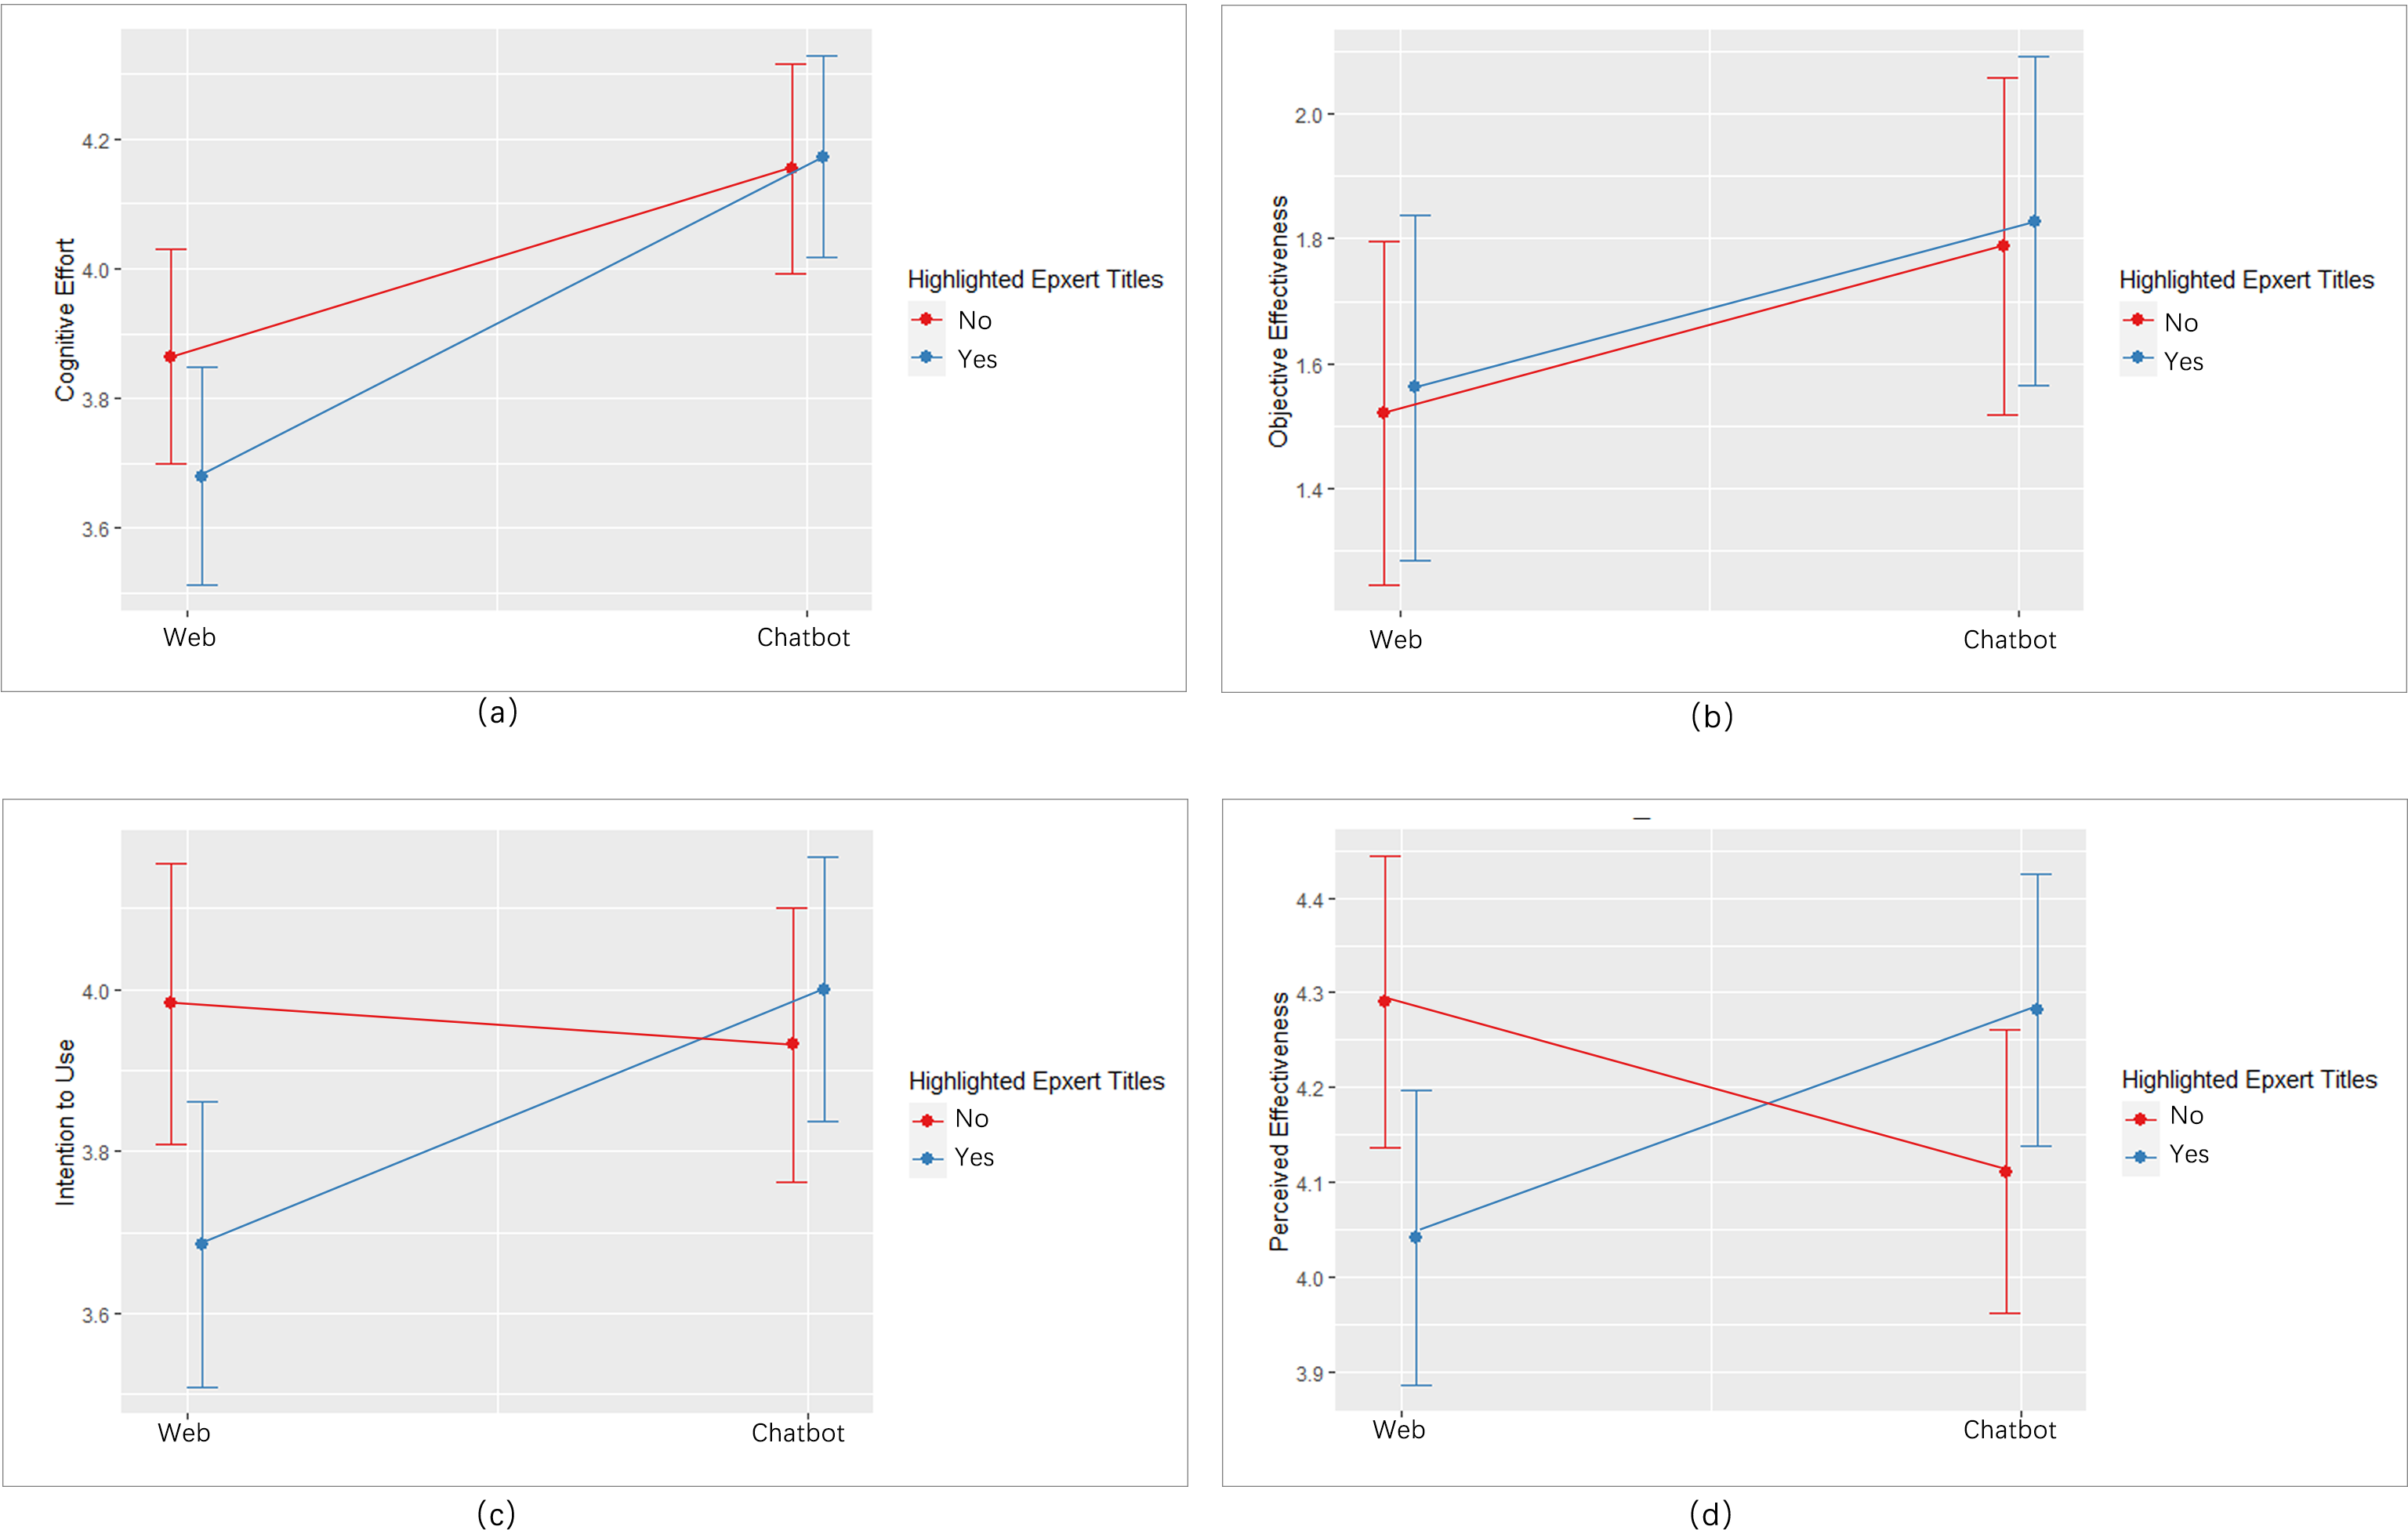
\includegraphics[width=\textwidth,height=4.6in]{figs/fig_main_interaction.png}
        \caption{The results of nonparametric factorial ANOVA.The interaction type has a significant main effect on (a) cognitive effects and a weak main effect on (b) objective effectiveness. 
        The chatbot is more likely to reduce users' cognitive effort and improve the actual effectiveness of correction.
        Two significant intention effects exist between interaction type and currection format on (c) perceived effectiveness and (d) intention to use.}
        \label{FIG:interaction}
    \end{figure*}

\subsection{Evaluation of Currection Effectiveness}
To comprehensively measure the correction effectiveness, we evaluated the experimental conditions from both subjective and objective aspects.
The results revealed an interaction effect in subjective effectiveness, while there was no significant difference in actual effectiveness.

\subsubsection{Perceived Effectiveness}
The 2*2 ANOVA shows a significant interaction effect between interaction type and format on perceived effectiveness, F(1, 323)=6.31, p<0.05, $\eta^{2}$=0.020.
We can observe that when participants use the web for fact-checking, the emphasis on expert titles decreases their perceived effectiveness.
However, there is an opposite trend when using the chatbot(see Figure~\ref{FIG:interaction}(d)).
Besides, the Chatbot*Highlighted design has a similar level of perceived effectiveness with the Web*Regualr(Table~\ref{tab:descriptive}).

\subsubsection{ Objectiveness Effectiveness}

Table~\ref{tab:descriptive} shows the participants' performance on the objective effectiveness questions. 
Participants answered the same questions in both tests, and we measured objective effectiveness by the increased number of correct answers to objective questions.
It can be seen that participants had better performance in the chatbot condition, while there was no significant effect on whether or not the expert title was highlighted.
In the web condition, participants' correct responses increased by 1.51 and 1.57 in the "Regular" and the "Highlighted" conditions, while in the chatbot condition, the increases were 1.79 and 1.82, respectively.
The results of two-way ANOVA show a weak significant main effect on the interaction type.

\subsection{Evaluation of Users' Intention}
We examine the impact of the tool on user's behavioral tendencies from both their intention to use this tool and their intention to fact-check it in the future.
Before that we measured the cognitive effort of users in different experimental conditions.
As mentioned before, people are not willing to spend extra cognitive effort to verify the authenticity of information. If the design can help users reduce the cognitive effort, this may have a positive impact on their behavioral tendencies, which is the reason we measured this variable.
There, higher values of the variable indicate easier of use and less cognitive effort.

\subsubsection{Cognitive Effort}
Analysis of cognitive effort yields a significant main effect of interaction type, F(1, 323)=20.239, p < 0.001, $\eta^{2}$ = 0.059, indicating that participants expend less cognitive effort to check facts when using chatbots compared to using the web(see Figure~\ref{FIG:interaction}(a)). 
The results do not show a significant main effect of format or an interaction effect.

\subsubsection{Intention to Use}
The main effects of interaction type and format are not found, but the interaction effect is significant, F (1, 323) = 5.310, p < 0.05, $\eta^{2}$ =0.022. 
Participants in the highlighted format reported lower intention to use than in the normal format condition when they use the web, but this effect disappears under the chatbot condition(see Figure~\ref{FIG:interaction}(b)).
There is no significant difference between the regular and highlighted formats when the chatbot is applied. Besides, the chatbot*highlighted design leads to the highest intention to use(Mean=3.993,SD=0.680).

\section{Discussion}
\subsection{Background}




\printcredits

%% Loading bibliography style file
% \bibliographystyle{model1-num-names}
\bibliographystyle{cas-model2-names}
% Loading bibliography database
\bibliography{cas-refs}


%\vskip3pt


\end{document}

